\subsection{Stabilitätsbedingung des doppeltsphärischen Aufbaus}
Die Messdaten zur Stabilitätsbedingung des doppeltsphärischen Aufbaus sind in Tabelle \ref{tab:stabsphere} notiert.
\begin{table}[h!]
  \centering
  \caption{Messdaten zu Überprüfung der Stabilitätsbedingung des doppelspärischen Aufbaus}
  \label{tab:stabsphere}
  \begin{tabular}{c c c c}
    \toprule
%    \multicolumn{3}{c}{$f_{\text{1& theo}}=\SI{0,1}{m}$} & \multicolumn{3}{c}{$f_{\text{2& theo}}=\SI{0,05}{m}$}\\
      L/m & I/mA & L/m & I/mA \\
      \midrule
      0,59  & 0,50464 & 0,99  & 0,40644 \\
      0,63  & 0,46055 & 1,03  & 0,32881 \\
      0,67  & 0,46578 & 1,07  & 0,27833 \\
      0,71  & 0,46251 & 1,11  & 0,26431 \\
      0,75  & 0,54064 & 1,15  & 0,23698 \\
      0,79  & 0,53707 & 1,19  & 0,24564 \\
      0,83  & 0,56027 & 1,23  & 0,016685\\
      0,87  & 0,53085 & 1,27  & 0,22631 \\
      0,91  & 0,44278 & 1,31  & 0,21110 \\
      0,95  & 0,42519 & 1,35  & 0,29335 \\
    \bottomrule
  \end{tabular}
\end{table}

%\end{landscape}
%\end{document}

Die Resonatorlänge $L$ ist in Abbildung \ref{fig:stabsphere} gegen den aufgenommenen Strom $I$ des Photodetektors aufgetragen.
\begin{figure}
  \centering
  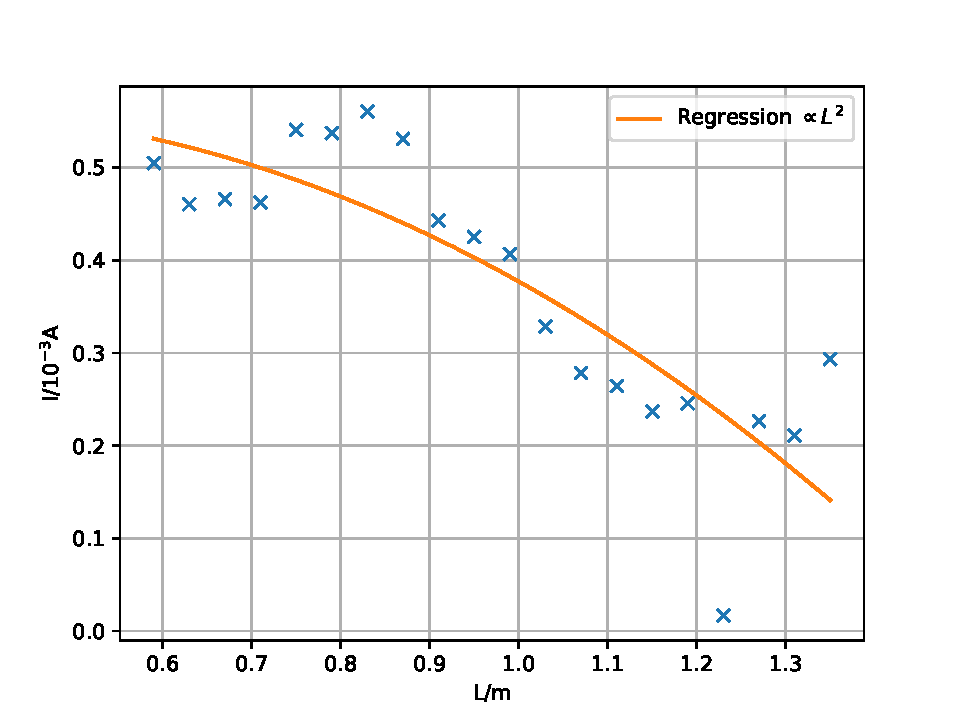
\includegraphics[width=\textwidth]{stabsphere.pdf}
  \caption{Überprüfung der Stabilitätsbedingung beim doppeltsphärischen Aufbau}
  \label{fig:stabsphere}
\end{figure}
Aus der Stabilitätsbedingung folgt der Zusammenhang
\begin{equation*}
  I=\left(1-\frac{L}{r_1} \right) \left(1- \frac{L}{r_2} \right).
\end{equation*}
Es wird folgende Funktion mit Python 3.6.3 (scipy.optimize, curve$\_$fit) gefittet:
\begin{equation*}
  I= \frac{a(L+b)^2}{r_1 r_2}+\frac{c(L+b)}{r_1 r_2}+\frac{d}{r_1 r_2}.
\end{equation*}
Es ergeben sich die Parameter
\begin{align*}
a &=& \SI{ -0.77   \pm 0.86 }{A} \\
b &=&(\SI{  1  }{} \pm \SI{1e+06 }{}) \si{m} \\
c &=&(\SI{  2  }{} \pm \SI{1e+06 }{}) \si{Am} \\
d &=&(\SI{ -0.3}{} \pm \SI{2e+06 }{}) \si{Am^2}. \\
\end{align*}
%
%\begin{align*}
%a &=& \SI{  -0.7701953 \pm 8.55242891e-01 }{A} \\
%b &=& \SI{  1.01713845 \pm 1.01457068e+06 }{m} \\
%c &=& \SI{  2.05577951 \pm 1.56283636e+06 }{Am} \\
%d &=& \SI{ -0.27390834 \pm 2.08573475e+06 }{Am^2} \\
%\end{align*}
%
\FloatBarrier

\subsection{Stabilitätsbedingung des sphärisch-flachen Aufbaus}
Die Messwerte zum Photodetektorstrom $I$ und der Resonatorlänge $L$ sind in Tabelle \ref{tab:stabflat} aufgenommen.
Aufgrund einer technischen Gegebenheit wird die Messung doppelt durchgeführt.
\begin{table}[h!]
  \centering
  \caption{Messdaten zu Überprüfung der Stabilitätsbedingung des sphärisch-flachen Aufbaus}
  \label{tab:stabflat}
  \begin{tabular}{c c c c}
    \toprule
    \multicolumn{2}{c}{Erste Messung} & \multicolumn{2}{c}{Zweite Messung}\\
      L/m & I/$\mu$A & L/m & I/$\mu$A \\
      \midrule
      0,57 & 5,0286  & 0,55 & 62,856 \\
      0,59 & 3,6969  & 0,57 & 62,001 \\
      0,63 & 10,6174 & 0,59 & 44,406 \\
      0,67 & 1,9912  & 0,61 & 45,883 \\
      0,71 & 0,38304 & 0,63 & 67,950 \\
      0,75 & 2,2791  & 0,65 & 50,739 \\
      0,79 & 5,5241  & 0,67 & 37,018 \\
      0,83 & 6,1024  & 0,69 & 13,102 \\
          &          & 0,71 & 25,690 \\
          &          & 0,73 & 15,603 \\
          &          & 0,75 & 15,836 \\
    \bottomrule
  \end{tabular}
\end{table}

%\end{landscape}
%\end{document}

In Abbildung \ref{fig:stabflat} ist der Photodetektorstrom $I$ in Abhängigkeit der Resonatorlänge $L$ dargestellt.
\begin{figure}
  \centering
  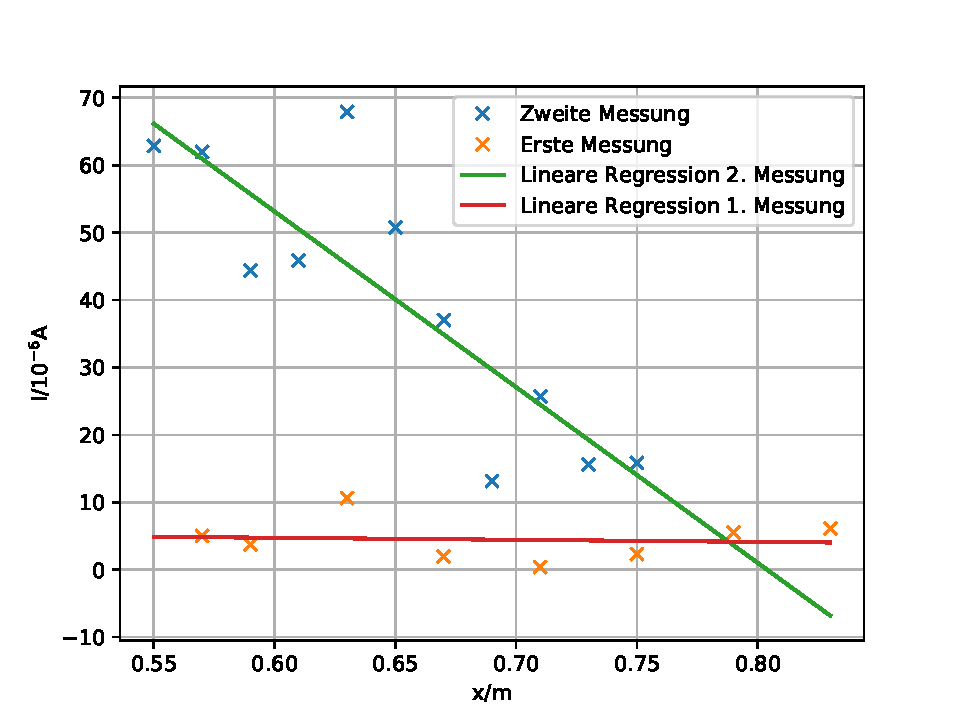
\includegraphics[width=\textwidth]{stabflat.pdf}
  \caption{Überprüfung der Stabilitätsbedingung beim sphärisch-flachen Aufbau}
  \label{fig:stabflat}
\end{figure}
Aufgrund des flachen Spiegels reduziert sich die Stabilitätsbedingung auf
\begin{equation*}
  I=\left(1-0 \right) \left(1- \frac{L}{r_2} \right)=1- \frac{L}{r_2}
\end{equation*}
Die lineare Regression hat die Form
\begin{equation*}
  I= aL+b
\end{equation*}
und wird erneut mit Python 3.6.3 (scipy.optimize, curve$\_$fit) durchgeführt.
Als Parameter ergeben sich:
\begin{align*}
&&\text{zweite Messung} \\
a &=& \SI{ -260 \pm 52 }{\frac{A}{m}} \\
b &=& \SI{  210 \pm 34 }{A} \\
&&\text{erste Messung} \\
a &=& \SI{ -3.0 \pm 13.7 }{\frac{A}{m}} \\
b &=& \SI{  6.6 \pm 9.6 }{A} \\
\end{align*}
%
%\begin{align*}
%&&\text{zweite Messung} \\
%a &=& \SI{ -260.60636539 \pm 52.34111607 }{\frac{A}{m}} \\
%b &=& \SI{  209.49268296 \pm 34.18239586 }{A} \\
%&&\text{erste Messung} \\
%a &=& \SI{ -3.03299421 \pm 13.67909208 }{\frac{A}{m}} \\
%b &=& \SI{  6.55319099 \pm 9.54894695 }{A} \\
%\end{align*}
%
\FloatBarrier

\subsection{Grundmode}
In Tabelle \ref{tab:grundmode} sind die Messwerte zur Intensitätsverteilung notiert.
\begin{table}[h!]
  \centering
  \caption{Messdaten zu Untersuchung der Grundmode}
  \label{tab:grundmode}
  \begin{tabular}{c c c c}
    \toprule
%    \multicolumn{2}{c}{Erste Messung} & \multicolumn{2}{c}{Zweite Messung}\\
      L/m & I/$\mu$A & L/m & I/$\mu$A \\
      \midrule
       0,031  &  0,01837  &  -0,003  &  1,68402 \\
       0,025  &  0,01850  &  -0,006  &  1,42631 \\
       0,020  &  0,03517  &  -0,009  &  1,00125 \\
       0,015  &  0,09141  &  -0,012  &  0,55967 \\
       0,012  &  0,22460  &  -0,015  &  0,24617 \\
       0,009  &  0,53102  &  -0,020  &  0,05179 \\
       0,006  &  0,97390  &  -0,025  &  0,02391 \\
       0,003  &  1,38290  &  -0,031  &  0,01991 \\
       0,000  &  1,63817  &    & \\
    \bottomrule
  \end{tabular}
\end{table}

%\end{landscape}
%\end{document}

Die Messwerte sind in Abbildung \ref{fig:grundmode} gegeneinander aufgetragen.
\begin{figure}
  \centering
  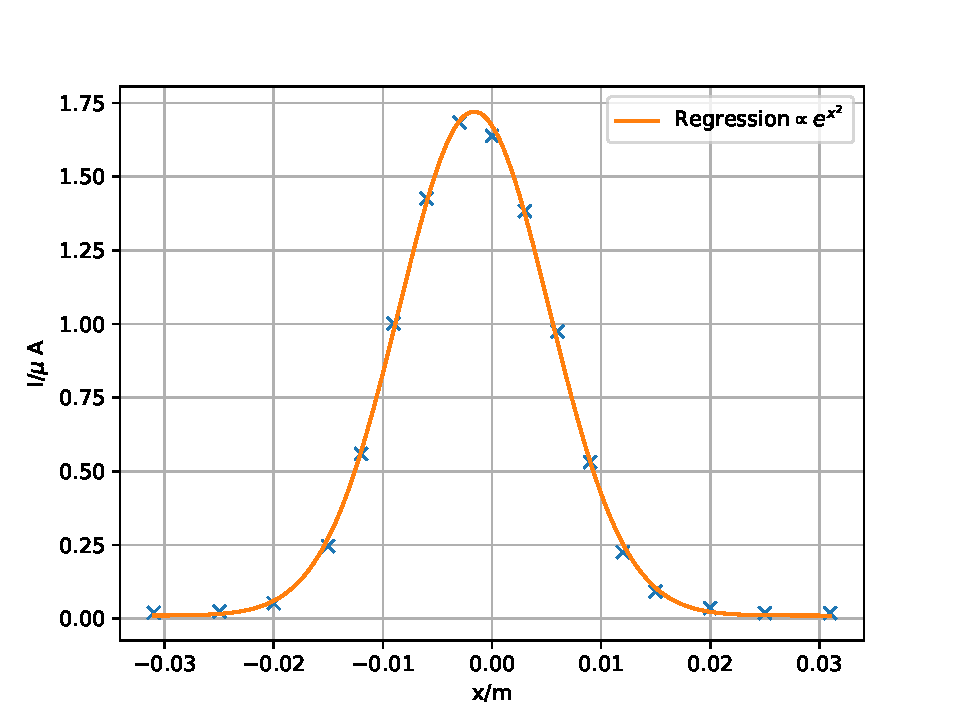
\includegraphics[width=\textwidth]{grundmode.pdf}
  \caption{Intensitätsverteilung der Grundmode}
  \label{fig:grundmode}
\end{figure}
Die Funktion
\begin{equation*}
  I= a \exp{\left( -b(x-c)^2 \right)}+d
\end{equation*}
wird mittels Python 3.6.3 (scipy.optimize, curve$\_$fit) an die Werte gefittet.
Es ergeben sich die Parameter
\begin{align*}
a &=& \SI{  1.710 \pm 0.014 }{A}\\
b &=& \SI{  10472 \pm 226 }{\frac{1}{m^2}}\\
c &=& \SI{ -0.00164 \pm 0.00006 }{m}\\
d &=& \SI{  0.01008 \pm 0.00857 }{A}.\\
\end{align*}
%
%\begin{align*}
%a &=& \SI{  1.71042311e+00 \pm 1.41925274e-02 }{A}\\
%b &=& \SI{  1.04714595e+04 \pm 2.25989252e+02 }{\frac{1}{m^2}}\\
%c &=& \SI{ -1.64149557e-03 \pm 5.87544034e-05 }{m}\\
%d &=& \SI{  1.00787408e-02 \pm 8.56648623e-03 }{A}.\\
%\end{align*}
%
Der Parameter $b$ entspricht nun
\begin{align*}
                  &&&&&      b &=&  \frac{2}{\omega^2} \\
  \Leftrightarrow &&&&& \omega &=& \pm \sqrt{\frac{2}{b}} \\
  \Rightarrow      &&&&& \omega &=& \pm \SI{ 0.01382 \pm 0.00015 }{m}\\
\end{align*}
Physikalisch ist nur das positive Ergebnis des Strahlradius $\omega$ sinnvoll.
%\omega &=& \pm \SI{ 0.0138201064795 \pm 0.00014912895026 }{m}
%\begin{equation*}
%\omega= \omega_{0} \sqrt{1+ (\frac{\lambda z}{\pi})^2}
%\end{equation*}
%
%\textbf{ERGEBNIS?\\
%$\omega_0$ (Strahltaille) berechnen?}
\FloatBarrier

\subsection{Erste Mode}
Die Messwerte zur Untersuchung der ersten transversalen Mode sind in Tabelle \ref{tab:erstemode} notiert.
\begin{table}[h!]
  \centering
  \caption{Messdaten zu Untersuchung der ersten Mode}
  \label{tab:erstemode}
  \begin{tabular}{c c c c c c c c c c c c c c c c c}
    \toprule
%    \multicolumn{2}{c}{Erste Messung} & \multicolumn{2}{c}{Zweite Messung}\\
      L/m & I/nA & L/m & I/nA & L/m & I/nA & L/m & I/nA \\
      \midrule
       0,031  &  0,62978 & 0,014  &  18,897  &  0,000   &  3,566  & -0,014  &  13,895  \\
       0,029  &  0,48938 & 0,013  &  20,22   &  -0,001  &  1,637  & -0,015  &  10,420  \\
       0,027  &  2,24440 & 0,012  &  24,974  &  -0,002  &  1,031  & -0,016  &  8,870   \\
       0,025  &  0,92853 & 0,011  &  28,676  &  -0,003  &  2,950  & -0,017  &  6,652   \\
       0,023  &  2,68534 & 0,010  &  35,051  &  -0,004  &  6,667  & -0,018  &  3,354   \\
       0,022  &  5,0257  & 0,009  &  39,979  &  -0,005  &  11,173 & -0,019  &  2,127   \\
       0,021  &  6,2573  & 0,008  &  43,685  &  -0,006  &  16,513 & -0,020  &  1,442   \\
       0,020  &  5,2613  & 0,007  &  44,221  &  -0,007  &  20,980 & -0,021  &  0,673   \\
       0,019  &  3,6343  & 0,006  &  40,383  &  -0,008  &  23,424 & -0,022  &  0,441   \\
       0,018  &  4,0211  & 0,005  &  34,308  &  -0,009  &  27,747 & -0,023  &  0,426   \\
       0,018  &  1,1202  & 0,004  &  24,899  &  -0,010  &  26,445 & -0,025  &  0,501   \\
       0,017  &  8,8913  & 0,003  &  18,409  &  -0,011  &  24,102 & -0,027  &  0,431   \\
       0,016  &  14,7981 & 0,002  &  12,210  &  -0,012  &  21,381 & -0,029  &  0,621   \\
       0,015  &  18,0773 & 0,001  &  7,091   &  -0,013  &  17,631 & -0,031  &  0,859   \\

    \bottomrule
  \end{tabular}
\end{table}

%\end{landscape}
%\end{document}

In Abbildung \ref{fig:erstemode} sind die Messwerte gegeneinander aufgetragen.
\begin{figure}
  \centering
  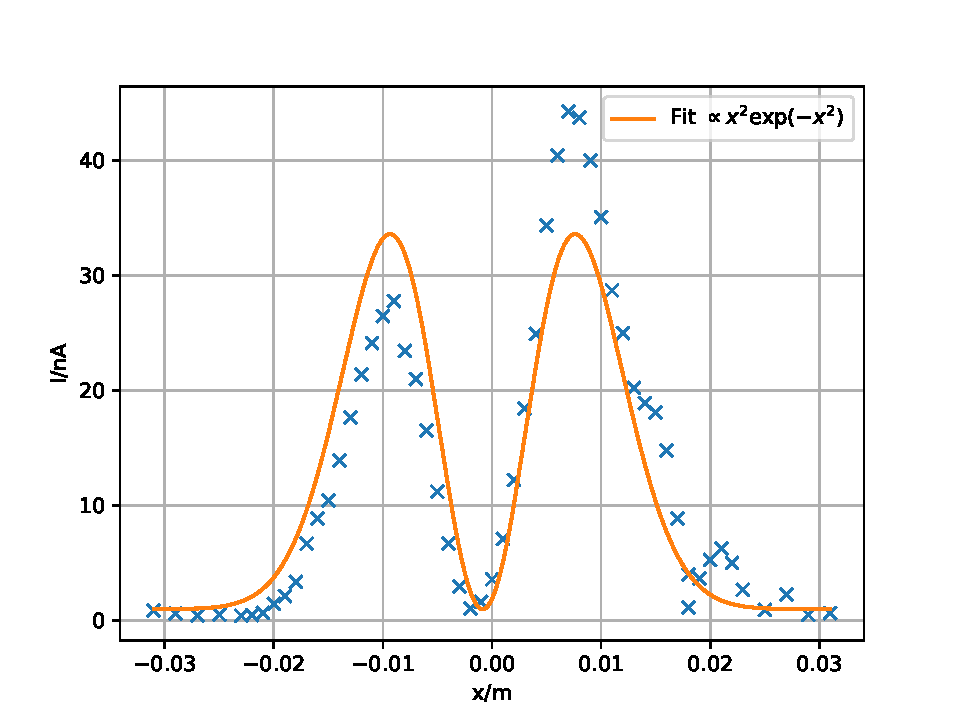
\includegraphics[width=\textwidth]{erstemode.pdf}
  \caption{Intensitätsverteilung der ersten Mode}
  \label{fig:erstemode}
\end{figure}
Es wird die Funktion
\begin{equation*}
  I = \frac{8 a (x-b)^2}{\omega^2} \quad \exp{ \left( \frac{-2d(x-b)^2}{\omega^2} \right)}+c
\end{equation*}
gefittet, die sich aus der Feldverteilung des Resonators mit den ersten Laguerrepolynomen ergibt.
Als Parameter ergeben sich:
\begin{align*}
  a      &=& \SI{  2700 \pm 2844377790 }{A} \\
  b      &=& \SI{ -0.00086 \pm 0.00023 }{m} \\
  c      &=& \SI{  0.98 \pm 1.14 }{A} \\
  d      &=& \SI{  122 \pm 128428998 }{} \\
  \omega &=& \SI{  0.13 \pm 69748.88 }{} .\\
\end{align*}
%
%\begin{align*}
%  a      &=& \SI{  2.70039879e+03 \pm 2.84437779e+09 }{A} \\
%  b      &=& \SI{ -8.60265803e-04 \pm 2.27043799e-04 }{m} \\
%  c      &=& \SI{  9.78796910e-01 \pm 1.13970356e+00 }{A} \\
%  d      &=& \SI{  1.21928078e+02 \pm 1.28428998e+08 }{} \\
%  \omega &=& \SI{  1.32436551e-01 \pm 6.97488774e+04 }{} .\\
%\end{align*}
%
\FloatBarrier

\subsection{Polarisation}
Die Messwerte zur Messreihe der Polarisation sind in Tabelle \ref{tab:polarisation} notiert.
\begin{table}[h!]
  \centering
  \caption{Messdaten zu Polarisation des Laserstrahls}
  \label{tab:polatisation}
  \begin{tabular}{c c c c}
    \toprule
%    \multicolumn{2}{c}{Erste Messung} & \multicolumn{2}{c}{Zweite Messung}\\
      $\sigma$/° & I/$\mu$ A & $\sigma$/° & I/$\mu$ A \\
      \midrule
        0 & 10,560 &   200 &  6,670 \\
       20 & 12,060 &   220 &  6,410 \\
       40 & 25,370 &   240 & 10,780 \\
       60 & 37,610 &   244 & 17,430 \\
       80 & 25,070 &   260 &  7,560 \\
      100 & 12,970 &   280 &  5,310 \\
      120 &  3,030 &   300 &  2,590 \\
      140 &  0,103 &   320 &  0,273 \\
      146 &  0,020 &   328 &  0,020 \\
      160 &  0,440 &   340 &  0,737 \\
      180 &  2,460 &   360 &  0,584 \\
    \bottomrule
  \end{tabular}
\end{table}

%\end{landscape}
%\end{document}

Die Polarisation $\sigma$ ist in Abbildung \ref{fig:polarisation} gegen den Photodetektorstrom $I$ aufgetragen.
\begin{figure}
  \centering
  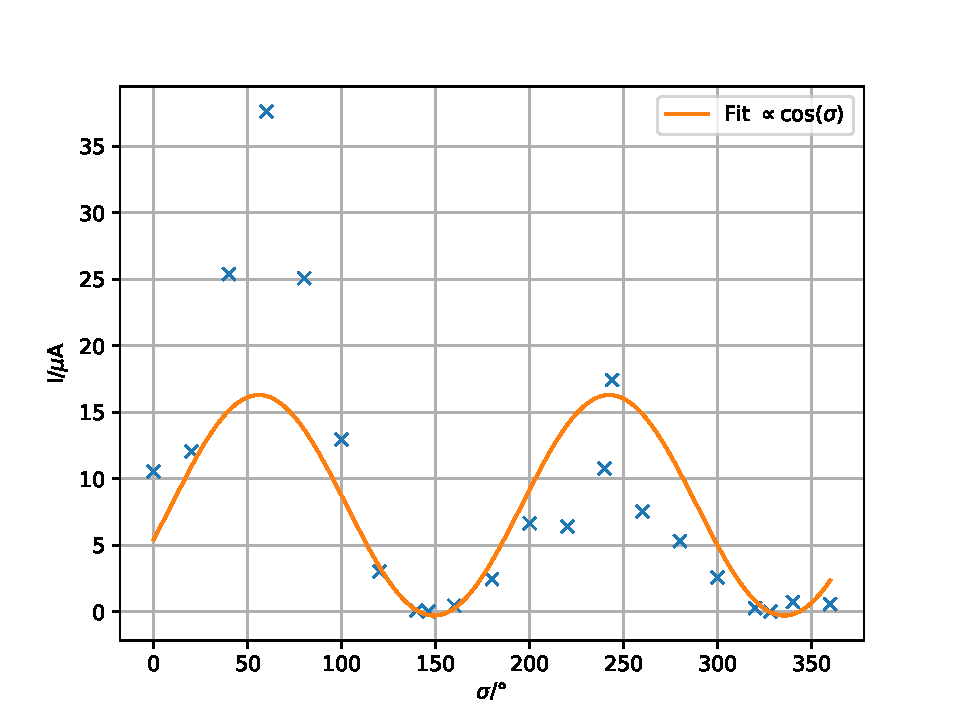
\includegraphics[width=\textwidth]{polarisation.pdf}
  \caption{Intensität in Abhängigkeit der Polarisation am Filter}
  \label{fig:polarisation}
\end{figure}
Es wird ein Fit der Form
\begin{equation*}
  I= a \sin{(b \sigma +c)}+d
\end{equation*}
durchgeführt.
Als Parameter ergeben sich
\begin{align*}
  a &=& \SI{ 8.3 \pm 1.6 }{nA} \\
  b &=& \SI{ 0.0337 \pm 0.0019 }{} \\
  c &=& \SI{ 5.97 \pm 0.38 }{°} \\
  d &=& \SI{ 8.01 \pm 1.19 }{nA}. \\
\end{align*}
%
%\begin{align*}
%  a &=& \SI{ 8.29329958 \pm 1.57797558 }{nA} \\
%  b &=& \SI{ 0.03369334 \pm 0.00188426 }{} \\
%  c &=& \SI{ 5.97045848 \pm 0.37691664 }{°} \\
%  d &=& \SI{ 8.00719666 \pm 1.18571944 }{nA}. \\
%\end{align*}
%
Die Extrema liegen bei den Polarisationen
\begin{align*}
  &\sigma_{\text{max, Fit}} &=&& \SI{50.97 \pm 0.38}{°},   && \SI{230.97 \pm 0.38}{°} \\
  &\sigma_{\text{max, Wert}} &=&& \SI{ 60 }{°},                          && \SI{ 244 }{°} \\
  &\sigma_{\text{min, Fit}} &=&& \SI{140.97 \pm 0.38}{°},  && \SI{320.97 \pm 0.38}{°} \\
  &\sigma_{\text{min, Wert}} &=&& \SI{ 146 }{°},                         && \SI{ 328 }{°}. \\
\end{align*}
\FloatBarrier

\subsection{Berechnung der Wellenlänge des Lasers}
Zur Berechnung der Wellenlänge wird im Interferenzmuster des Gitters der Abstand des ersten Nebenmaximum zum Hauptmaximum notiert.
Außerdem wird der Abstand des Gitters zum Schirm notiert.
\begin{align*}
\text{Ordnung des Maximums}                        && n &=&\SI{1}{}&&\\
\text{Abstand Hauptmaximum - 1. Nebenmaximum}      && d &=&\SI{0.052 \pm 0.002}{m} && \\
\text{Abstand Gitter - Schirm}                     && L &=&\SI{0.807 \pm 0.002}{m} && \\
\text{Abstand der Gitterlinien}                    && a &=&\SI{1e-05}{m} && \\
\end{align*}
Es ergibt sich folgende Wellenlänge:
\begin{equation*}
    \lambda = \frac{a}{n} \sin{\left( \arctan{\left( \frac{d}{L} \right)} \right)} = \SI{6.43e-07}{m} = \SI{643.0 \pm 0.3}{nm}.
\end{equation*}
Der Fehler wird als Gaussfehler berechnet:
\begin{align*}
  \Delta \lambda &=& \sqrt{ \left( \frac{aL}{ \left( L^2 + d^2 \right) \sqrt{ \frac{d^2}{L^2} + 1 }} \right)^2 \cdot \left(\Delta d \right)^2 + \left( \frac{-ad}{ \left( d^2 + L^2 \right) \sqrt{ \frac{d^2}{L^2} + 1 }} \right)^2 \cdot \left( \Delta L \right)^2 } &&\\
                 &=& \SI{0.3}{nm}. &&
\end{align*}
